%%
% BIThesis 研究生学位论文模板 The BIThesis Template for Graduate Thesis
% This file has no copyright assigned and is placed in the Public Domain.
%%

\chapter{面向轻量化本地部署的参数高效本体约束知识抽取方法}
\label{chap:lightweight-ke}

\section{问题描述}

\section{参数高效的本体约束知识抽取流程}

参数高效的本体约束知识抽取方法是一种结合大语言模型领域适配能力与领域本体约束机制的知识抽取方法。这种方法首先利用参数高效微调技术，使基座模型具备对领域文本的理解与实体关系联合抽取能力；随后，在模型生成候选结果的基础上，结合领域本体规则对抽取结果进行约束、筛选与重排序，从而输出更加稳定、更加符合领域结构要求的知识结果。

\begin{figure}[htbp]
  \centering
  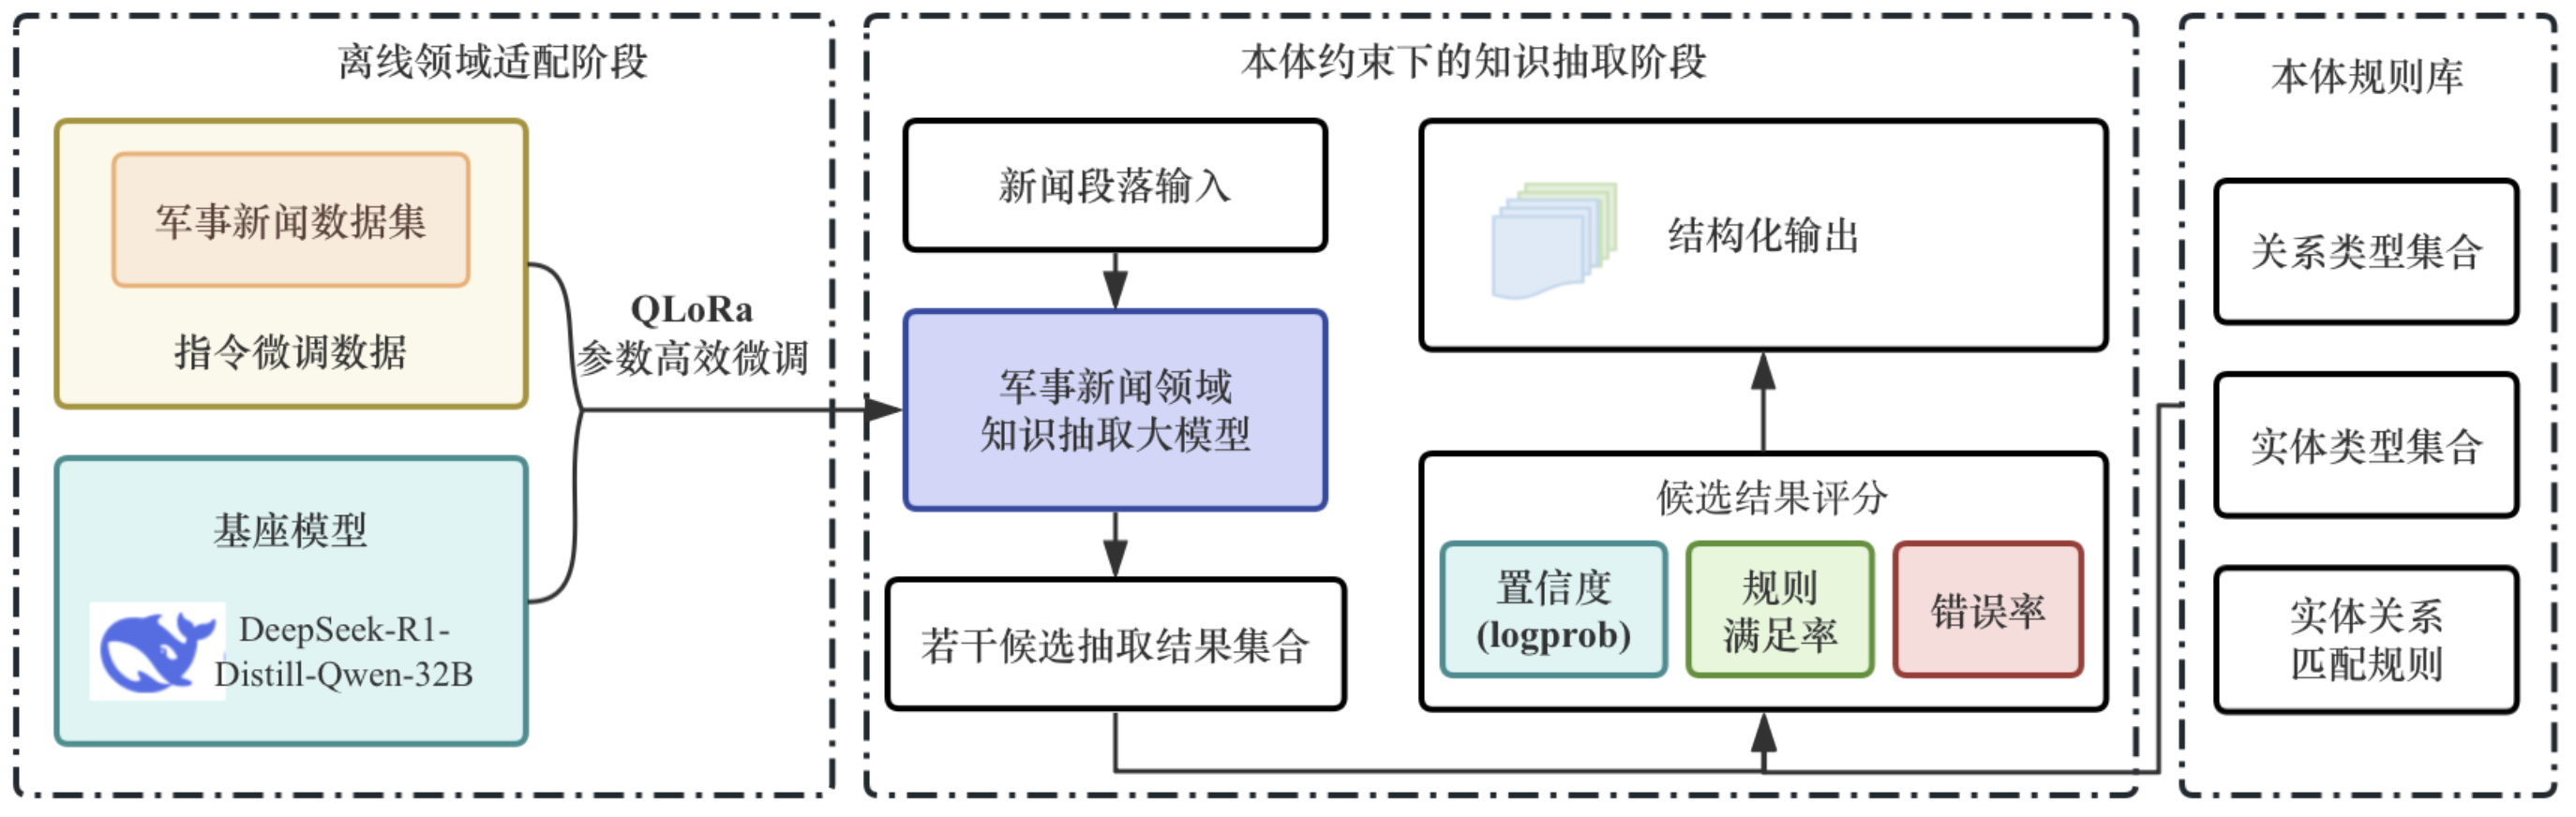
\includegraphics[width=0.95\textwidth]{figures/参数高效本体约束抽取流程图.png}
  \caption{参数高效的本体约束知识抽取流程}
  \label{fig:efficient_ontology_constrained_extraction_process}
\end{figure}

图~\ref{fig:efficient_ontology_constrained_extraction_process}展示了参数高效本体约束抽取的整体流程。该流程主要分为四个阶段：离线领域适配、候选结果生成、本体约束与候选评分、结构化输出。以下是每个阶段的详细说明：

\begin{enumerate}
\item 离线领域适配阶段：在这个阶段需要收集和整理用于模型微调的指令数据，所使用到的训练数据主要来源于上一章节基于自建军事新闻语料构建的银标数据集，需要将其进一步组织为适用于指令微调的训练样本。在此基础上，选取开源大语言模型 DeepSeek-R1-Distill-Qwen-32B 作为基座模型，并采用 QLoRA 训练策略进行参数高效微调。通过冻结原始参数、对模型权重进行低比特量化，并在部分线性层中引入低秩适配矩阵，可以在较低训练开销下完成领域知识抽取能力的适配，使得方法适用于各种显卡算力及显存容量有限的环境，大大拓展了本章方法的应用范围。
\item 候选结果生成：在完成领域适配后，将新闻段落输入到知识抽取模型中，由模型根据任务指令生成结构化的抽取结果。与单次确定性生成方式不同，本章方法针对同一输入文本采用受控随机采样策略生成若干个候选抽取结果集合。每个候选结果集合均对应一次完整的实体关系联合抽取结果，包含实体之间的关系信息和用于后续结构化组织的属性信息。通过生成多个候选结果，可以为后续结果筛选提供更充分的比较空间。
\item 本体约束与候选评分：在候选结果生成后，需要结合本体规则对抽取结果进行进一步分析，包括关系类型集合、实体类型集合以及实体和关系之间的匹配规则。对于每个候选结果，分别从模型置信度、本体规则满足度以及错误项数量三个方面进行综合评分。其中模型置信度由生成序列的 logprob 给出，规则满足率用于衡量候选结果中关系与本体约束的一致程度，错误项则主要包括重复三元组、格式错误问题。经过归一化处理后，上述指标共同构成候选结果的综合得分。
\item 结构化输出：在完成候选评分之后，选取得分最高的候选结果作为最终输出结果，并以统一的结构化 JSON 形式返回。通过这一过程，模型输出结果不再仅依赖单次生成，而是在领域适配、本体规则约束与候选结果选择的共同作用下得到进一步校正，这样不仅可以提升抽取结果的稳定性和结构合法性，也能够减少不合理三元组和错误关系的产生。
\end{enumerate}

\subsection{基于 QLoRA 的领域适配}

为了使模型具备更好的领域知识抽取能力，需要对开源大语言模型进行领域适配。本章的核心思路是：基于前文构建的银标数据，组织面向军事新闻知识抽取任务的指令微调数据集，再结合参数高效微调技术 QLoRA，对基座模型进行低成本的任务适配，使其能够理解军事新闻文本中的领域表达，并按照指令输出结构化的抽取结果。

\subsubsection*{（1）指令数据的构建}

构建高质量指令数据是实现领域知识抽取的基础，训练数据需要覆盖军事新闻中的主要实体类型和关系类型，还需要尽量保证输出结果具有统一的结构化形式，便于后续进行规则过滤、候选比较以及图谱入库处理。

相较于直接使用通用领域信息抽取数据，在自建军事新闻语料库上构建的数据可以更好地反映军事新闻领域里的高频实体、关系表达及其组合模式，模型在训练阶段就能够接触到大量符合军事新闻领域特点的抽取实例，从而更好地学习领域术语、事件叙事模式以及结构化输出要求之间的对应关系。本章从上一章构建的银标数据中选择了五种实体类型，包括新闻事件实例（MilitaryNewsEvent）、行动主体（Actor）、军事资产（MilitaryAsset）、地理位置（Location）和时间（Time），以及四种关系类型，包括hasActor、hasMilitaryAsset、hasLocation 和 hasTime。

训练数据集以新闻段落作为基本输入粒度，每条训练样本主要由三个部分组成：

1）\textbf{任务指令}：用于明确当前任务是军事新闻文本的实体关系联合抽取任务，并规定输出需要满足结构化结果的组织要求；

2）\textbf{输入文本}：即待抽取的军事新闻段落文本，作为模型进行语义理解知识抽取的依据；

3）\textbf{目标输出}：由数据集的抽取结果转换得到，用于指导模型学习从新闻段落到实体关系结果的映射过程。

以下是一个示例训练样本的任务指令和输入文本样例：

\begin{lstlisting}[style=promptbox]
你是一个军事新闻领域的实体关系抽取模型。我将给你一条由”””分割的新闻报道，请根据要求抽取出以下实体和关系。
军事新闻实体关系定义：
MilitaryNewsEvent hasActor Actor 新闻事件相关的行动、参与或接收主体
MilitaryNewsEvent hasMilitaryAsset MilitaryAsset 新闻事件相关的军事资产
MilitaryNewsEvent hasLocation Location 新闻事件发生或影响的地理位置 
MilitaryNewsEvent hasTime Time 新闻事件的发生、计划时间或报道中的时间表达
其中，MilitaryNewsEvent包含属性：事件ID（event_id，从新闻开头截取）和事件类型（event_type），事件类型包含deploy（部署）、exhibit（展示）、experiment（实验）、manoeuvre（演习）、accident（事故）、conflict（冲突）、support（支援）七类。
操作步骤：
 (1) 阅读文献：仔细阅读并理解提供的新闻报道内容。
 (2) 实体识别：在文献中识别出新闻事件实例（MilitaryNewsEvent）、行动主体（Actor）、军事资产（MilitaryAsset）、地理位置（Location）和时间（Time）。
 (3) 关系抽取：基于识别的实体，建立它们之间的上述关系。
任务约束：
 (1) 如果不存在某类型的关系，则无需给出。
 (2) 请一步一步思考。
输出格式：
JSON，形如[ {"predicate": "hasActor","subject": {"MilitaryNewsEvent": {"event_id": "E1", "event_type": "support"} },"object": {"Actor": "乌克兰"} }, {"predicate": "hasMilitaryAsset","subject": {"MilitaryNewsEvent": {"event_id": "E1", "event_type": "support"} },"object": {"MilitaryAsset": "新型战术弹道导弹"} }, ...]
新闻报道：
"""E1据乌克兰政府网站消息，当地时间1月11日，乌克兰国防部表示，英国将为乌克兰研发新型战术弹道导弹，以增强乌克兰的火力..."""
JSON:
\end{lstlisting}

通过这种方式，可以将上一章已经构建完成的银标数据自然衔接到基座模型的训练流程中，以便逐步学习军事新闻文本中的术语表达、叙事模式以及结构化输出要求之间的对应关系。

\subsubsection*{（2）基座模型选择}

本文采用了大语言模型 DeepSeek-R1-Distill-Qwen-32B 作为领域适配的基础模型。该模型属于开源的预训练模型，是由 DeepSeek 团队通过 “知识蒸馏”（Knowledge Distillation） 技术，基于 Qwen2.5-32B 架构蒸馏而成，具备较好的中英文文本理解与生成能力，能够为后续的领域任务适配提供稳定的语言基础，同时还具有较低的部署成本，采用INT4量化即可在24GB显存的GPU上进行本地推理，更便于在本地环境下进行训练、推理和部署。

DeepSeek团队 在 DeepSeek-R1 的论文中提出了一个关键结论：推理模式是可以被“蒸馏”的，如果直接把大模型（R1）产生的优秀推理步骤喂给小模型（Qwen）吃，小模型的推理能力会瞬间大幅提升，甚至超过那些自己尝试用强化学习（RL）训练的小模型。而本章选用的DeepSeek-R1-Distill-Qwen-32B 模型就是把 DeepSeek-R1 的能力提取出来，灌输给了 Qwen-2.5-32B，从而让这个较小的模型也获得了类似 R1 的深度思考能力。

\begin{table}[htbp]
  \centering
  \caption{DeepSeek-R1 与 DeepSeek-R1-Distill-Qwen-32B 特性对比}
  \label{tab:deepseek_r1_vs_distill_qwen32b}
  {\renewcommand{\arraystretch}{1.18}
  \small
  \setlength{\tabcolsep}{4pt}
  \begin{tabularx}{0.98\textwidth}{
    >{\raggedright\arraybackslash}p{0.12\textwidth}
    >{\raggedright\arraybackslash}p{0.31\textwidth}
    >{\raggedright\arraybackslash}X
  }
    \toprule
    模型 & DeepSeek-R1-671B & DeepSeek-R1-Distill-Qwen-32B \\
    \midrule
    训练方式
    & 大规模强化学习（RL）+ 冷启动数据
    & 监督微调（SFT），直接学习 R1 的输出 \\

    基座模型
    & DeepSeek-V3-Base
    & Qwen-2.5-32B \\

    优势
    & 思维能力很高，能自我进化
    & 性价比高，在 32B 尺寸下拥有接近671B模型的推理能力 \\

    训练消耗
    & 非常昂贵的算力消耗
    & 相对极低 \\
    \bottomrule
  \end{tabularx}}
\end{table}

表~\ref{tab:deepseek_r1_vs_distill_qwen32b}对 DeepSeek-R1 与 DeepSeek-R1-Distill-Qwen-32B 的特性进行了对比，可以看出后者在训练方式、基座模型、优势和代价等方面都具有明显的轻量化特点，非常适合本文的研究需求。

\subsubsection*{（3）QLoRA 训练策略}

对于参数规模较大的大语言模型而言，全参数微调（Full Fine-tuning）的显存占用和训练成本极高，32B参数级别的大模型进行常规全量微调需要超过448GB的GPU内存，这对于大多数研究者来说是难以承受的。即使采用混合精度（如16位或8位）微调，仍然需要数百GB的显存。然而，低秩自适应（Low-Rank Adaption, LoRA）技术能够在几乎不降低模型性能以及不产生推理延迟的情况下，通过仅微调模型的一小部分参数来达到与全参数微调相似的效果。QLoRA 在 LoRA 的基础上引入了几项新的技术，包括：1）一种新的数据类型 4-bit NormalFloat（NF4），该数据类型在理论上是正态分布权重的信息优化；2）双量化（Double Quantization），对量化常量再次进行量化来减少存储需求；3）分页优化器（Paged Optimizer），管理内存峰值。图~\ref{fig:different_fine_tuning_methods_comparison} 展示了全参数微调、LoRA 微调和 QLoRA 微调在训练方式上的对比，可以看出 QLoRA 在保持较高性能的同时，显著降低了训练成本，使得大语言模型的领域适配变得更加可行和高效。

\begin{figure}[htbp]
  \centering
  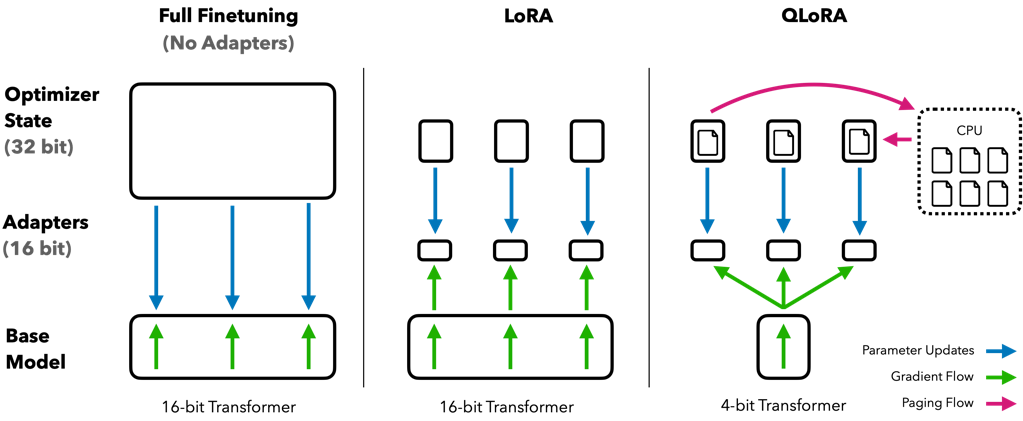
\includegraphics[width=0.95\textwidth]{figures/不同的微调方法对比.png}
  \caption{不同的微调方法对比}
  \label{fig:different_fine_tuning_methods_comparison}
\end{figure}

QLoRA 的基本思想可以概括为以下三个方面：

1）\textbf{冻结原始参数}：在训练过程中，不直接更新基座模型的大部分预训练参数，而是将这些参数作为稳定的语言知识底座保留下来，从而避免全参数优化所带来的高计算代价；

2）\textbf{低比特量化}：将基座模型权重以低比特形式进行压缩表示，以减少显存占用，降低较大参数规模模型的训练门槛；

3）\textbf{低秩适配矩阵}：在模型的部分线性层中引入可训练的低秩矩阵，用于学习下游任务所需的参数增量，使模型能够在不改变原始大规模参数的前提下完成对军事新闻抽取任务的适配。

本章方法会对基座模型进行量化处理，并在指定层中插入可训练的低秩适配矩阵，再基于前文构建好的军事新闻指令微调样本，对这些新增参数进行监督训练，从而得到一个能够根据新闻段落输入生成结构化抽取结果的 Student 端基础模型。通过这种方式，模型可以在较低的训练成本下获得对军事新闻文本实体关系联合抽取任务的能力，也为后续引入本体约束和多候选结果选择奠定了模型基础。

\subsection{领域本体模型约束}

本体模型约束的主要内容即对候选抽取结果进行合法性检查与结果过滤，将模型输出限制在已有 schema 所允许的结构空间内，减少关系越界、类型和格式错误的问题。

\subsubsection*{（1）本体模型约束}

本章的本体约束对象，是由单个新闻报道片段生成的候选结果集合，系统会重点检查以下三个方面：1）实体类型是否合法，判断结果中的实体类型是否属于领域本体预先定义的实体集合；2）关系类型是否合法，判断结果中的关系标签是否属于预定义的关系集合。3）关系连接是否合法：判断一条关系两端的实体类型，即“头实体类型—关系类型—尾实体类型”是否满足领域本体规定的连接方式。为了统一表示，可将领域本体中允许的合法连接关系记为
\[
\Omega=\{(T_h,r,T_t)\},
\]
其中，$T_h$ 表示头实体类型，$r$ 表示关系类型，$T_t$ 表示尾实体类型。对于任意候选三元组 $(e_h,r,e_t)$，若满足
\[
(type(e_h),r,type(e_t))\in\Omega,
\]
则认为该三元组在结构上满足本体约束；否则，将其视为不合法结果。这个判断过程直接通过预先整理好的类型匹配规则自动完成。

\subsubsection*{（2）结构合法性约束}

在经过本体模型约束的评估后，系统还会执行以下几个步骤：1）结构完整性检查，判断候选结果是否满足统一结构化输出的基本要求，避免因字段缺失或者结构残缺而影响后续处理；2）异常结果检查，识别重复三元组、实体边界异常，排除会影响结果质量的问题。

\subsubsection*{（3）约束作用}

本体约束在本章中的作用，主要体现在两个方面。

1）\textbf{保证结果结构合法}：通过显式的类型匹配规则，将模型输出限制在领域本体允许的关系空间内，减少非法关系和不合理连接；

2）\textbf{提升结果可用性}：经过本体约束处理后的候选结果，在结构一致性和规范性都会更稳定，便于后续在此基础上进行候选排序。

需要说明的是，本节的本体约束并不直接决定最终输出结果，只是为后续候选结果的选择提供基础，而最终从多个候选中选择哪一个，需要在下一小节结合多候选结果生成与评分机制进一步完成。

\subsection{多候选结果生成与评分}

为降低单次生成结果的随机波动，同一输入新闻段落将采用受控随机采样方式生成多个候选结果集合，并进一步结合模型置信度、本体规则满足度和错误惩罚项进行综合评分，选取得分最高的候选作为最终输出，从而在保持生成多样性的同时，尽量选出结构更稳定、规则更一致、错误更少的抽取结果。

\subsubsection*{（1）多候选结果生成}

对于每一段输入文本，本文使用经过领域适配后的知识抽取模型进行多次独立解码，得到 $K$ 个候选抽取结果，记为
\[
\mathcal{Y}=\{Y_1,Y_2,\dots,Y_K\},
\]
其中每个 $Y_k$ 表示该输入对应的一个完整抽取结果集合，内部包含若干实体、关系以及相应属性信息，并统一组织为结构化 JSON 三元组形式。

为了实现候选结果的生成，需要采用 top-$p$ 采样（nucleus sampling）作为解码策略。其基本思想是：在生成每一个 token 时，先按照概率从高到低对候选 token 排序，再选取累计概率达到阈值 $p$ 的最小 token 集合，最后只在这一集合中进行采样，不会直接在全部词表上进行随机采样，这样可以避免从概率过低的 token 中随意采样，同时保留一定的生成灵活性，图~\ref{fig:top_p_sampling}是一个简单的示意图。相较于贪心解码，top-$p$ 采样能够得到更加多样的候选结果；相较于完全无约束的随机采样，它又能将生成过程控制在较高概率区域内，因此更适合生成多个合理的候选结果集合，为后续的比较和选择提供更丰富的备选项。

\begin{figure}[htbp]
  \centering
  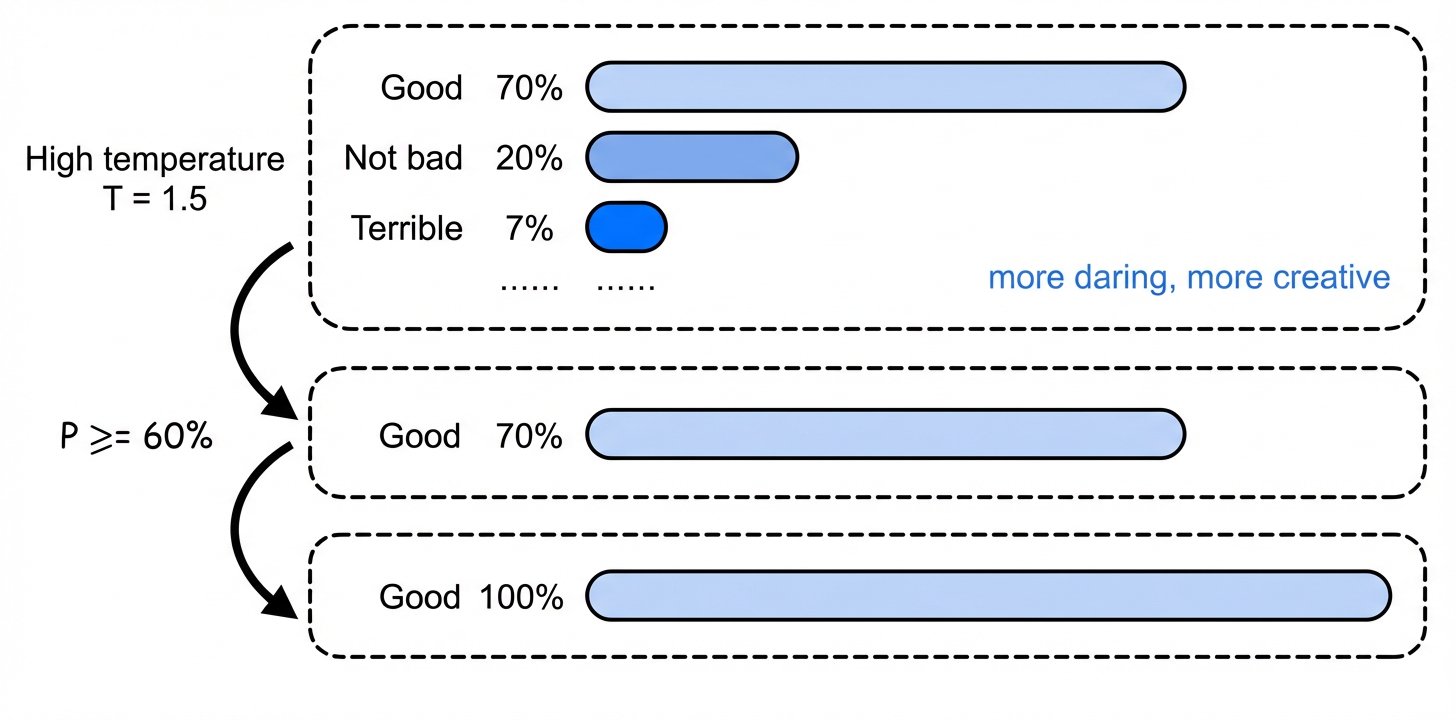
\includegraphics[width=0.75\textwidth]{figures/top-p示意图.png}
  \caption{top-$p$ 采样示意图}
  \label{fig:top_p_sampling}
\end{figure}

若将当前时刻的候选 token 概率分布记为 $\{q_1,q_2,\dots\}$，并按概率从高到低排序，则 top-$p$ 采样对应的候选集合可写为
\[
V_p=\left\{x_1,x_2,\dots,x_m \,\middle|\, \sum_{i=1}^{m} q_i \ge p \right\},
\]
其中 $V_p$ 表示当前步用于采样的 nucleus 集合。模型仅在该集合内进行下一 token 的生成。

在本文中，一个候选结果的比较单位是“一次完整输出”，而不是其中的某个局部关系。这是因为实体关系联合抽取结果具有整体结构特征，同一候选内部的实体识别、关系判断和属性组织通常相互关联。若只对单个三元组独立处理，容易破坏整体结果的一致性；而以完整结果集合作为比较对象，更符合后续结构化解析和图谱入库的处理方式。

需要说明的是，若某次生成结果能够被解析为合法 JSON，但输出为空列表 \texttt{[]}，则说明该次解码未抽取出任何有效三元组。对于这类空结果，本文将其直接从候选集合中剔除，不再进入后续评分与候选选择过程。

\subsubsection*{（2）模型置信度计算}

得到多个候选结果之后，需要首先衡量每个候选结果本身的生成可信程度。本文采用生成序列的 logprob 作为候选结果的基础置信度信号。

这里的 logprob 指的是模型在生成某个输出序列时，对该序列中各个 token 所赋予概率的对数值之和。设候选结果 $Y_k$ 对应的输出序列为 $(y_1,y_2,\dots,y_n)$，则其序列 logprob 可表示为
\[
\log P(Y_k)=\sum_{t=1}^{n}\log P(y_t \mid y_{<t},x),
\]
其中 $x$ 表示输入新闻段落，$y_{<t}$ 表示当前位置之前已经生成的 token。直观地说，若某个候选结果的 logprob 较高，说明模型在当前输入条件下更倾向于生成该结果。

由于不同候选结果的序列长度可能不同，若直接比较总 logprob，长序列往往会因为累积项更多而天然偏低。因此，本文对 logprob 做长度归一化处理，将其转化为候选结果的置信度分量 $Conf_k$。一种简单做法是采用平均 token 对数概率，即
\[
Conf_k=\frac{1}{n}\sum_{t=1}^{n}\log P(y_t \mid y_{<t},x).
\]
通过这种方式，可以在不同长度的候选结果之间进行相对公平的比较。

\subsubsection*{（3）规则满足度与错误惩罚项}

仅依靠模型置信度并不足以选出最适合入库的结果，还需要进一步考虑候选结果与领域本体规则的一致性。设候选结果 $Y_k$ 中共包含 $N_k$ 个关系三元组，其中满足本体约束规则的三元组数量为 $M_k$，则其规则满足率定义为
\[
Rule_k=
\begin{cases}
\frac{M_k}{N_k}, & Y_k \text{ 可解析且 } N_k>0, \\
0, & Y_k \text{ 不可解析}.
\end{cases}
\]
其本体约束规则主要依据第三章中已经定义好的实体类型集合、关系类型集合以及实体类型—关系类型—实体类型匹配规则进行检查。若候选结果中存在较多关系越界或类型不匹配情况，该项得分就会较低。

除了本体约束规则满足情况，还需要关注到结果中存在的结构性错误。本文主要考虑以下两类错误：1）重复三元组，即同一候选结果中存在经字符串标准化后头实体、关系类型和尾实体三项完全一致的重复记录；2）格式错误，即输出不符合预设 JSON 结构，导致结果无法被解析器正确解析。

设候选结果 $Y_k$ 中重复三元组的数量为 $Dup_k$，格式错误指示变量定义为
\[
Fmt_k=
\begin{cases}
1, & Y_k \text{ 非合法 JSON}, \\
0, & \text{正常可解析}.
\end{cases}
\]
定义重复错误率为
\[
DupRate_k=
\begin{cases}
\frac{Dup_k}{N_k}, & Y_k \text{ 可解析且 } N_k>0, \\
0, & Y_k \text{ 不可解析}.
\end{cases}
\]
则候选结果 $Y_k$ 的错误惩罚值定义为
\[
Error_k=\lambda_1 \cdot DupRate_k+\lambda_2 \cdot Fmt_k,\quad \lambda_1+\lambda_2=1,
\]
其中，$\lambda_1$ 和 $\lambda_2$ 分别表示重复错误项和格式错误项的惩罚权重。

\subsubsection*{（4）综合评分与最优结果选择}

为统一比较多个候选结果，需要从模型置信度、本体规则满足度和错误惩罚项三个方面构建综合评分函数。设经过空结果过滤后保留的候选集合为
\[
\mathcal{Y}'=\{Y_1,Y_2,\dots,Y_{K'}\},
\]
其中 $K'$ 表示过滤后剩余候选数量。为简化表示，下文对保留候选重新编号。由于 $Conf_k$、$Rule_k$ 和 $Error_k$ 原本不在同一量纲区间，需要在加权组合前先对三者进行归一化处理，分别记为 $\widetilde{Conf}_k$、$\widetilde{Rule}_k$ 和 $\widetilde{Error}_k$。对于任意指标 $Z_k \in \{Conf_k, Rule_k, Error_k\}$，采用最小—最大归一化方式：
\[
\widetilde{Z}_k=
\begin{cases}
\frac{Z_k-\min_{1\le j\le K'} Z_j}{\max_{1\le j\le K'} Z_j-\min_{1\le j\le K'} Z_j}, & \max_{1\le j\le K'} Z_j>\min_{1\le j\le K'} Z_j, \\
0, & \max_{1\le j\le K'} Z_j=\min_{1\le j\le K'} Z_j.
\end{cases}
\]
当某一指标在全部候选之间取值完全相同时，说明已不具备区分作用，因此将其归一化结果统一记为 0，不再对候选排序产生额外影响。

候选结果 $Y_k$ 的综合得分定义为
\[
Score_k=\alpha \cdot \widetilde{Conf}_k+\beta \cdot \widetilde{Rule}_k-\gamma \cdot \widetilde{Error}_k,
\quad \alpha+\beta+\gamma=1,\ \alpha,\beta,\gamma\ge 0,
\]

其中，$\alpha$、$\beta$ 和 $\gamma$ 分别表示模型置信度、本体规则满足度和错误惩罚项的权重系数。该公式对应的含义比较直接：候选结果的生成概率越高、越符合本体规则、包含的错误越少，则其最终得分越高。上述权重参数的具体取值在实验部分结合验证集调参结果进一步给出。

在此基础上，对候选集合 $\mathcal{Y}'$ 进行统一评分。若 $K'=0$，说明当前轮生成结果均为空，直接返回空结果；若 $K'=1$，则唯一保留候选直接作为最终输出；若 $K'>1$，则选取得分最高的候选作为最终输出，即
\[
Y^{*}=Y_{k^{*}},\quad k^{*}=\arg\max_{1\le k\le K'} Score_k.
\]

这样，最终输出将在多个候选结果之间经过比较后确定，能够在一定程度上缓解单次解码带来的随机性，使系统更倾向于保留置信度较高、规则更符合、错误更少的结果。

\section{实验设计}

\subsection{数据集与实验设置}

（需要介绍实验环境、实验用数据、模型微调参数设置）

\subsection{对比组与评价指标}

\subsection{实验结果与分析}

\section{本章小结}
